% 3D Bounding Box Regressor Architecture Figure
% Compile with: pdflatex bbox_regressor_architecture.tex

\documentclass{article}
\usepackage[paperwidth=30cm, paperheight=11cm, margin=0.5cm]{geometry}
\usepackage{tikz}
\usepackage{xcolor}
\usepackage{amsmath}

\usetikzlibrary{shapes.geometric, arrows.meta, positioning, calc, backgrounds, fit, decorations.pathreplacing}

% Define colors (colorblind-friendly palette)
\definecolor{convblue}{RGB}{55, 126, 184}
\definecolor{fcgreen}{RGB}{77, 175, 74}
\definecolor{outputorange}{RGB}{255, 127, 0}
\definecolor{inputgray}{RGB}{200, 200, 200}
\definecolor{dropoutred}{RGB}{228, 26, 28}

\pagestyle{empty}

\begin{document}
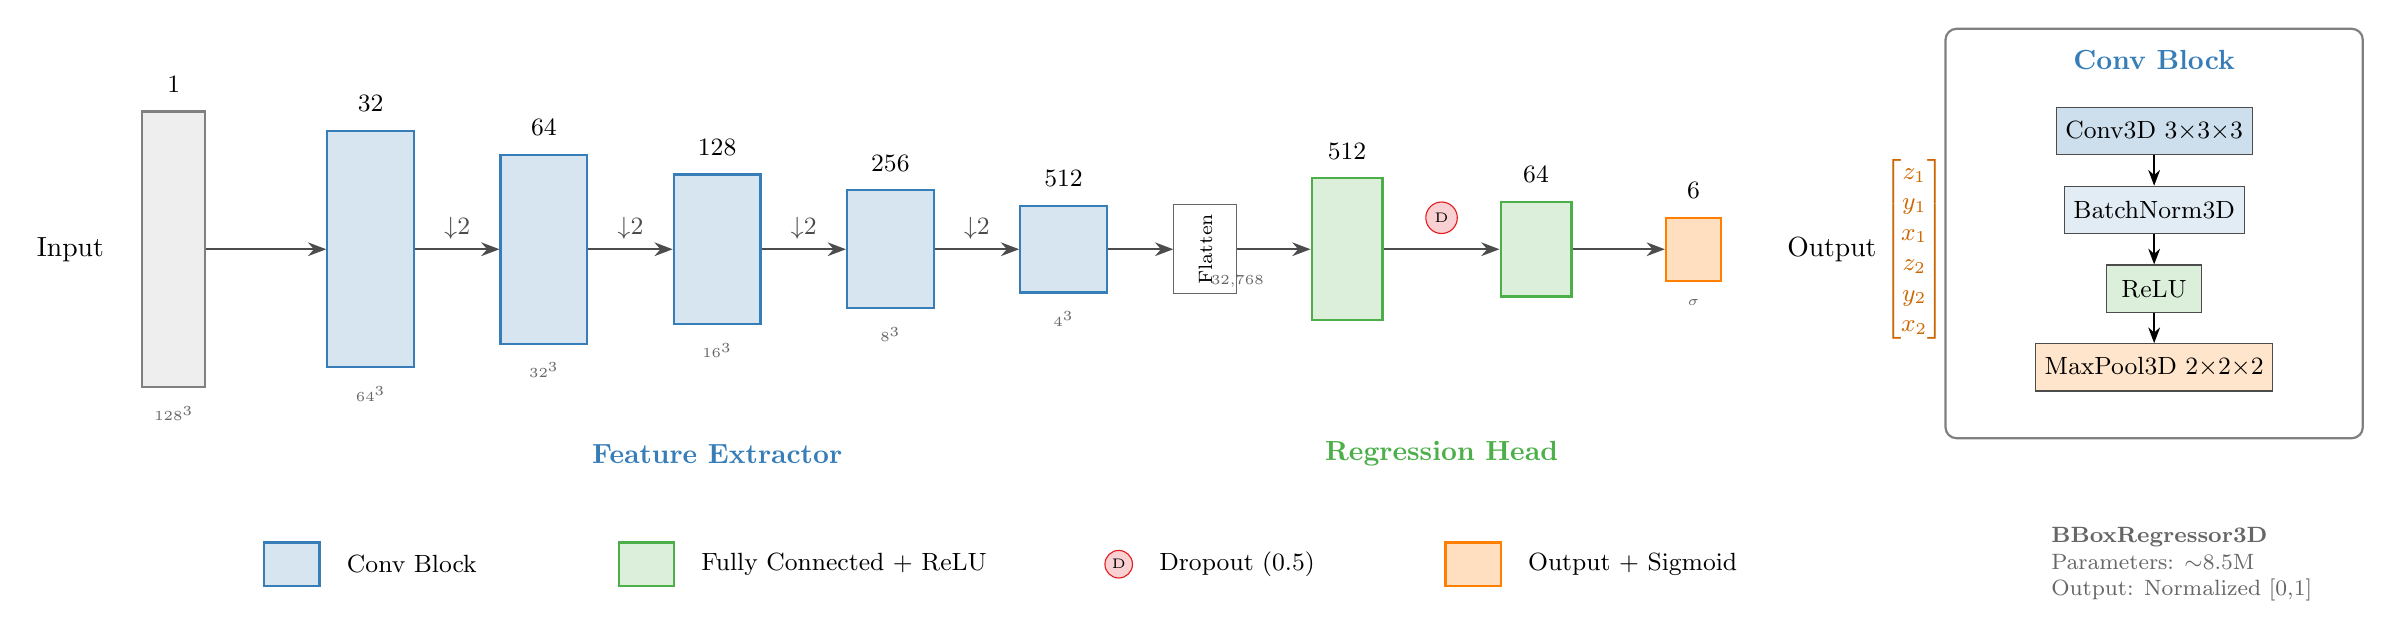
\begin{tikzpicture}[
    % Conv block style
    conv/.style={
        rectangle,
        draw=convblue,
        fill=convblue!20,
        line width=0.8pt,
        minimum width=1.1cm,
    },
    % FC block style
    fc/.style={
        rectangle,
        draw=fcgreen,
        fill=fcgreen!20,
        line width=0.8pt,
        minimum width=0.9cm,
    },
    % Output style
    outblock/.style={
        rectangle,
        draw=outputorange,
        fill=outputorange!25,
        line width=0.8pt,
        minimum width=0.7cm,
    },
    % Input style
    inblock/.style={
        rectangle,
        draw=black!50,
        fill=inputgray!30,
        line width=0.8pt,
    },
    % Arrow styles
    flow/.style={->, >=Stealth, thick, black!70},
    % Labels
    chanlabel/.style={font=\small, above=3pt},
    sizelabel/.style={font=\tiny, below=3pt, text=black!60},
]

% =====================================================
% INPUT
% =====================================================

\node[inblock, minimum height=3.5cm, minimum width=0.8cm] (input) at (-1.5, 0) {};
\node[chanlabel] at (input.north) {1};
\node[sizelabel] at (input.south) {$128^3$};
\node[left=10pt of input, font=\normalsize] {Input};

% =====================================================
% CONVOLUTIONAL BLOCKS (heights represent spatial dimensions)
% =====================================================

% Block 1: 128 -> 64, 1ch -> 32ch
\node[conv, minimum height=3.0cm] (c1) at (1.0, 0) {};
\node[chanlabel] at (c1.north) {32};
\node[sizelabel] at (c1.south) {$64^3$};

% Block 2: 64 -> 32, 32ch -> 64ch
\node[conv, minimum height=2.4cm] (c2) at (3.2, 0) {};
\node[chanlabel] at (c2.north) {64};
\node[sizelabel] at (c2.south) {$32^3$};

% Block 3: 32 -> 16, 64ch -> 128ch
\node[conv, minimum height=1.9cm] (c3) at (5.4, 0) {};
\node[chanlabel] at (c3.north) {128};
\node[sizelabel] at (c3.south) {$16^3$};

% Block 4: 16 -> 8, 128ch -> 256ch
\node[conv, minimum height=1.5cm] (c4) at (7.6, 0) {};
\node[chanlabel] at (c4.north) {256};
\node[sizelabel] at (c4.south) {$8^3$};

% Block 5: 8 -> 4, 256ch -> 512ch
\node[conv, minimum height=1.1cm] (c5) at (9.8, 0) {};
\node[chanlabel] at (c5.north) {512};
\node[sizelabel] at (c5.south) {$4^3$};

% =====================================================
% FLATTEN
% =====================================================

\node[rectangle, draw=black!60, fill=white, minimum width=0.5cm, minimum height=0.8cm, font=\scriptsize, rotate=90] (flat) at (11.6, 0) {Flatten};
\node[sizelabel, below=6pt of flat] {32,768};

% =====================================================
% FC LAYERS
% =====================================================

% FC1: 32768 -> 512
\node[fc, minimum height=1.8cm] (fc1) at (13.4, 0) {};
\node[chanlabel] at (fc1.north) {512};

% Dropout indicator
\node[circle, draw=dropoutred, fill=dropoutred!20, minimum size=0.4cm, font=\tiny, inner sep=0pt] (drop) at (14.6, 0.4) {D};

% FC2: 512 -> 64
\node[fc, minimum height=1.2cm] (fc2) at (15.8, 0) {};
\node[chanlabel] at (fc2.north) {64};

% FC3: 64 -> 6
\node[outblock, minimum height=0.8cm] (fc3) at (17.8, 0) {};
\node[chanlabel] at (fc3.north) {6};
\node[sizelabel] at (fc3.south) {$\sigma$};

% =====================================================
% OUTPUT VISUALIZATION
% =====================================================

% Output box representation
\node[right=20pt of fc3, font=\normalsize] {Output};

% Bounding box coordinate labels
\node[right=55pt of fc3, font=\small, text=outputorange!80!black] (coords) {
    $\begin{bmatrix} z_1 \\ y_1 \\ x_1 \\ z_2 \\ y_2 \\ x_2 \end{bmatrix}$
};

% =====================================================
% FLOW ARROWS
% =====================================================

% Input to conv blocks
\draw[flow] (input.east) -- (c1.west);
\draw[flow] (c1.east) -- (c2.west) node[midway, above, font=\small] {$\downarrow$2};
\draw[flow] (c2.east) -- (c3.west) node[midway, above, font=\small] {$\downarrow$2};
\draw[flow] (c3.east) -- (c4.west) node[midway, above, font=\small] {$\downarrow$2};
\draw[flow] (c4.east) -- (c5.west) node[midway, above, font=\small] {$\downarrow$2};

% Conv to flatten to FC
\draw[flow] (c5.east) -- (flat.north);
\draw[flow] (flat.south) -- (fc1.west);
\draw[flow] (fc1.east) -- (fc2.west);
\draw[flow] (fc2.east) -- (fc3.west);

% =====================================================
% SECTION LABELS
% =====================================================

\node[font=\normalsize\bfseries, convblue] at (5.4, -2.6) {Feature Extractor};
\node[font=\normalsize\bfseries, fcgreen] at (14.6, -2.6) {Regression Head};

% =====================================================
% CONV BLOCK DETAIL INSET
% =====================================================

\begin{scope}[shift={(21.5, 1.0)}, scale=1.0]
    % Inset box
    \draw[black!50, thick, rounded corners=4pt] (-0.5, -3.4) rectangle (4.8, 1.8);
    \node[font=\normalsize\bfseries, convblue] at (2.15, 1.4) {Conv Block};

    % Conv3D
    \node[rectangle, draw=black!70, fill=convblue!25, minimum width=2.0cm, minimum height=0.6cm, font=\small] (cb_conv) at (2.15, 0.5) {Conv3D 3$\times$3$\times$3};

    % BatchNorm
    \node[rectangle, draw=black!70, fill=convblue!15, minimum width=1.6cm, minimum height=0.6cm, font=\small] (cb_bn) at (2.15, -0.5) {BatchNorm3D};

    % ReLU
    \node[rectangle, draw=black!70, fill=fcgreen!20, minimum width=1.2cm, minimum height=0.6cm, font=\small] (cb_relu) at (2.15, -1.5) {ReLU};

    % MaxPool
    \node[rectangle, draw=black!70, fill=outputorange!20, minimum width=1.8cm, minimum height=0.6cm, font=\small] (cb_pool) at (2.15, -2.5) {MaxPool3D 2$\times$2$\times$2};

    % Arrows
    \draw[->, >=Stealth, semithick] (cb_conv) -- (cb_bn);
    \draw[->, >=Stealth, semithick] (cb_bn) -- (cb_relu);
    \draw[->, >=Stealth, semithick] (cb_relu) -- (cb_pool);
\end{scope}

% =====================================================
% LEGEND
% =====================================================

\begin{scope}[shift={(0, -4.0)}]
    % Conv Block
    \node[conv, minimum height=0.55cm, minimum width=0.7cm] (l1) at (0, 0) {};
    \node[font=\small, right=6pt of l1] {Conv Block};

    % FC Layer
    \node[fc, minimum height=0.55cm, minimum width=0.7cm] (l2) at (4.5, 0) {};
    \node[font=\small, right=6pt of l2] {Fully Connected + ReLU};

    % Dropout
    \node[circle, draw=dropoutred, fill=dropoutred!20, minimum size=0.35cm, font=\tiny, inner sep=0pt] (l3) at (10.5, 0) {D};
    \node[font=\small, right=6pt of l3] {Dropout (0.5)};

    % Output
    \node[outblock, minimum height=0.55cm, minimum width=0.7cm] (l4) at (15.0, 0) {};
    \node[font=\small, right=6pt of l4] {Output + Sigmoid};
\end{scope}

% =====================================================
% MODEL INFO
% =====================================================

\node[font=\footnotesize, text=black!60, align=left] at (24.0, -4.0) {
    \textbf{BBoxRegressor3D}\\
    Parameters: $\sim$8.5M\\
    Output: Normalized [0,1]
};

\end{tikzpicture}
\end{document}
